%%This is a very basic article template.
%%There is just one section and two subsections.
\documentclass{article}
\usepackage[latin1]{inputenc} %coding of writteninput %latin1 allows for Umlaute
\usepackage[T1]{fontenc}%vectorized fonts (cm-super package)
\usepackage[german]{babel}%some specifics of the german language
\usepackage{amsfonts, amsmath, amsthm, amssymb, mathabx, paralist}
\setlength{\parindent}{0em} 
\usepackage{listings}
\usepackage{longtable}
\usepackage{pdfpages}
 \lstset{language=Matlab,%
    %basicstyle=\color{red},
    breaklines=true,%
    morekeywords={matlab2tikz},
    keywordstyle=\color{blue},%
    morekeywords=[2]{1}, keywordstyle=[2]{\color{black}},
    identifierstyle=\color{black},%
    stringstyle=\color{mylilas},
    commentstyle=\color{mygreen},%
    showstringspaces=false,%without this there will be a symbol in the places where there is a space
    numbers=left,%
    numberstyle={\tiny \color{black}},% size of the numbers
    numbersep=9pt, % this defines how far the numbers are from the text
    emph=[1]{for,end,break},emphstyle=[1]\color{red}, %some words to emphasise
    %emph=[2]{word1,word2}, emphstyle=[2]{style},    
}

 %Decisiontree
 \usepackage{tikz,forest}
 \usepackage{tikz}
\usetikzlibrary{arrows,shapes,snakes,automata,backgrounds,petri}
\usetikzlibrary{arrows.meta}
  
\usepackage{graphicx} 

\usepackage{verbatim}%f�r txt datei

\usepackage{color} %red, green, blue, yellow, cyan, magenta, black, white
\definecolor{mygreen}{RGB}{28,172,0} % color values Red, Green, Blue
\definecolor{mylilas}{RGB}{170,55,241}

\title{Homework 1}
\author{ Miriam Wagner\\373045}
\begin{document}
\maketitle


%\mainmatter
\section*{Question 1}
I used for solving this exercise Matlab (with my own written code no packages).
For the distance I used euclidian distance.

My clustering algorithm calculates for every Datavector the distances to
every centroid and then checks which centroid is closed. The vector is add to
the closest cluster. When all datavectors are put in a cluster the new cluster
centroids are calculated. 

My abort criterion is the change between the centroids. If they still change I
will apply the algorithms again. Because of the computer accuracy I do not use
0, but $10^{-15}$. I also let the algorithm stop after 3 rounds, but it would
end after 4 rounds, too.

After the first round all data is clustered in cluster 2 and 3. I decided to let
be the first centroid $(-1000,-1000,-1000)$. Than it does not influence the
result anymore. But two other options would be
\begin{enumerate}
  \item Set the centroid to 0 or 1 or do not change it
  \item random restart of just this or all cluster centroids
\end{enumerate}

I also did the random restart, then I get an other clustering. the steps in
between of the second version I did not write down here. The distances and
centroids are for the first version.

% Table generated by Excel2LaTeX from sheet 'Blad1'
\begin{table}[h]
  \centering
  \caption{Distances first round}
      \begin{tabular}{rrr}
    \multicolumn{1}{l}{distance\_to\_cluster\_1} & \multicolumn{1}{l}{distance\_to\_cluster\_2} & \multicolumn{1}{l}{distance\_to\_cluster\_3} \\
    43000,00002 & 3000,002694 & 23000,00899 \\
    35000,07642 & 5000,486525 & 15000,09671 \\
    26888,00021 & 13112,00189 & 6888,039561 \\
    44000,00413 & 4000,028178 & 24000,00035 \\
    40000,00664 & 20,15113235 & 20000,002 \\
    47500,00003 & 7500,000631 & 27500,00685 \\
    31000,02992 & 9000,088284 & 11000,02773 \\
    45000,0265 & 5000,212648 & 25000,02102 \\
    37000,00023 & 3000,000006 & 17000,00789 \\
    15000,23523 & 25000,12893 & 5000,409169 \\
    45000,00443 & 5000,027278 & 25000,00028 \\
    42500,00031 & 2500,000209 & 22500,00527 \\
    44000,00319 & 4000,02221 & 24000,00046 \\
    43500,00003 & 3500,002355 & 23500,00885 \\
    25000,03222 & 15000,04597 & 5000,051895 \\
    40000,00014 & 7,034833476 & 20000,01362 \\
    42200,02875 & 2200,477885 & 22200,02037 \\
    41500,00014 & 1500,016496 & 21500,01267 \\
    33000,00058 & 7000,000319 & 13000,00815 \\
    47000,00118 & 7000,004581 & 27000,0024 \\
    \end{tabular}%
  \label{tab:dist1}%
\end{table}%

% Table generated by Excel2LaTeX from sheet 'Blad1'
\begin{table}[ht]
  \centering
  \caption{centroids after first round}
    \begin{tabular}{rrr}
    \multicolumn{1}{l}{centroid\_1} & \multicolumn{1}{l}{centroid\_2} & \multicolumn{1}{l}{centroid\_3} \\
    -10000 & 8752,941176 & 27704 \\
    -10000 & 7,779844647 & 13,629704 \\
    -10000 & 22,82352941 & 44 \\
    \end{tabular}%
  \label{tab:centr1}%
\end{table}%

% Table generated by Excel2LaTeX from sheet 'Sheet2'
\begin{table}[ht]
  \centering
  \caption{Distances second round}
        \begin{tabular}{rrr}
    \multicolumn{1}{l}{distance\_to\_cluster\_1} & \multicolumn{1}{l}{distance\_to\_cluster\_2} & \multicolumn{1}{l}{distance\_to\_cluster\_3} \\
    22116,19085 & 1753,037892 & 20704,03917 \\
    28758,56529 & 6247,302602 & 12704,04405 \\
    36006,45169 & 14359,07461 & 4592,203257 \\
    21365,89781 & 2752,952894 & 21704,01257 \\
    24510,81085 & 1247,073587 & 17704,00916 \\
    18878,30691 & 6252,966011 & 25204,03083 \\
    32284,64122 & 10247,08985 & 8704,002232 \\
    20652,19999 & 3753,0757 & 22704,00565 \\
    27003,89625 & 4247,084395 & 14704,04516 \\
    47192,82789 & 26247,14247 & 7296,135236 \\
    20631,35796 & 3752,941811 & 22704,00875 \\
    22505,10872 & 1253,018169 & 20204,03122 \\
    21367,51278 & 2752,941595 & 21704,01232 \\
    21734,0764 & 2253,017414 & 21204,03843 \\
    37765,65939 & 16247,07449 & 2704,012108 \\
    24496,12265 & 1247,240632 & 17704,05272 \\
    22765,44019 & 953,4550448 & 19904,00236 \\
    23287,55072 & 253,8360288 & 19204,0486 \\
    30483,445 & 8247,069583 & 10704,05649 \\
    19220,80594 & 5752,946555 & 24704,01792 \\
    \end{tabular}%
  \label{tab:dist2}%
\end{table}%
% Table generated by Excel2LaTeX from sheet 'Sheet2'
\begin{table}[ht]
  \centering
  \caption{centroids second round}
    \begin{tabular}{rrr}
    \multicolumn{1}{l}{centroid\_1} & \multicolumn{1}{l}{centroid\_2} & \multicolumn{1}{l}{centroid\_3} \\
    -10000 & 8112,5 & 25528 \\
    -10000 & 7,029701813 & 15,1678105 \\
    -10000 & 21,4375 & 44,25 \\
    \end{tabular}%
  \label{tab:cent2}%
\end{table}%
% Table generated by Excel2LaTeX from sheet 'Sheet2'
\begin{table}[ht]
  \centering
  \caption{Distances third round}
    \begin{tabular}{rrr}
    \multicolumn{1}{l}{distance\_to\_cluster\_1} & \multicolumn{1}{l}{distance\_to\_cluster\_2} & \multicolumn{1}{l}{distance\_to\_cluster\_3} \\
    22116,19085 & 1112,627498 & 18528,04545 \\
    28758,56529 & 6887,73384 & 10528,0504 \\
    36006,45169 & 14999,51298 & 2416,39972 \\
    21365,89781 & 2112,51454 & 19528,01534 \\
    24510,81085 & 1887,5148 & 15528,01088 \\
    18878,30691 & 5612,522945 & 23028,03511 \\
    32284,64122 & 10887,53297 & 6528,001674 \\
    20652,19999 & 3112,67816 & 20528,00509 \\
    27003,89625 & 4887,517724 & 12528,05539 \\
    47192,82789 & 26887,5854 & 9472,102143 \\
    20631,35796 & 3112,502093 & 20528,01042 \\
    22505,10872 & 612,6238331 & 18028,03664 \\
    21367,51278 & 2112,50014 & 19528,0146 \\
    21734,0764 & 1612,589208 & 19028,04449 \\
    37765,65939 & 16887,51723 & 528,0438334 \\
    24496,12265 & 1887,603135 & 15528,0622 \\
    22765,44019 & 314,2232448 & 17728,00213 \\
    23287,55072 & 388,0020635 & 17028,05672 \\
    30483,445 & 8887,50778 & 8528,074443 \\
    19220,80594 & 5112,504053 & 22528,02049 \\
    \end{tabular}%
  \label{tab:dist3}%
\end{table}%
% Table generated by Excel2LaTeX from sheet 'Sheet2'
\begin{table}[ht]
  \centering
  \caption{centroids third round}
    \begin{tabular}{rrr}
    \multicolumn{1}{l}{centroid\_1} & \multicolumn{1}{l}{centroid\_2} & \multicolumn{1}{l}{centroid\_3} \\
    -10000 & 7520  & 23822,4 \\
    -10000 & 7,497431933 & 12,1369984 \\
    -10000 & 22,06666667 & 37,8 \\
    \end{tabular}%
  \label{tab:cent3}%
\end{table}%

\begin{align*}
\text{cluster} = \{2,2,3,2,2,2,3,2,2,3,2,2,2,2,3,2,2,2,3,2\} 
\end{align*}

Where the order of the vector is the order of the data. The second version has
the following clustering:
\begin{align*}
\text{clusterrandom} =\{ 2,1,3,2,2,2,1,2,1,3,2,2,2,2,3,2,2,2,1,2\}
\end{align*}

I would choose the second version over the first, because you have higher chance
of getting the clusters. But you do not know how many clusters to expect, so it
could be that there are just 2 clusters. What other steps would include a
preexamination to figure out how many clusters to expect. Also the centroids can
be choose on basis of the given data.

% % Table generated by Excel2LaTeX from sheet 'Blad1'
% \begin{table}[ht]
%   \centering
%   \caption{Cluster 1}
%     \begin{tabular}{rrr}
%     \multicolumn{1}{l}{amount\_req} & \multicolumn{1}{l}{case\_duration} & \multicolumn{1}{l}{total\_activities} \\
%           &       &  \\
%     \end{tabular}%
%   \label{tab:clust1}%
% \end{table}%
% % Table generated by Excel2LaTeX from sheet 'Blad1'
% \begin{table}[htbp]
%   \centering
%   \caption{Cluster 2}
%        \begin{tabular}{rrr}
%     \multicolumn{1}{l}{amount\_req} & \multicolumn{1}{l}{case\_duration} & \multicolumn{1}{l}{total\_activities} \\
%     7000  & 0,29309 & 6 \\
%     15000 & 28,43964 & 74 \\
%     6000  & 0,048206 & 25 \\
%     10000 & 12,95023 & 26 \\
%     2500  & 0,021134 & 7 \\
%     5000  & 29,51885 & 46 \\
%     13000 & 0,515625 & 10 \\
%     5000  & 7,612419 & 25 \\
%     7500  & 0,489861 & 11 \\
%     6000  & 6,503808 & 22 \\
%     6500  & 0,002049 & 6 \\
%     10000 & 0,000799 & 3 \\
%     7800  & 19,1099 & 52 \\
%     8500  & 0,000486 & 3 \\
%     3000  & 6,955382 & 15 \\
%     10000 & 0,000799 & 3 \\
%     7800  & 19,1099 & 52 \\
%     8500  & 0,000486 & 3 \\
%     17000 & 0,01375 & 12 \\
%     3000  & 6,955382 & 15 \\
%     \end{tabular}%
%   \label{tab:clust2}%
% \end{table}%
% % Table generated by Excel2LaTeX from sheet 'Blad1'
% \begin{table}[htbp]
%   \centering
%   \caption{Cluster 3}
%     \begin{tabular}{rrr}
%     \multicolumn{1}{l}{amount\_req} & \multicolumn{1}{l}{case\_duration} & \multicolumn{1}{l}{total\_activities} \\
%     23112 & 0,000532 & 3 \\
%     19000 & 19,78213 & 45 \\
%     35000 & 19,74352 & 88 \\
%     25000 & 21,14506 & 41 \\
%     17000 & 0,01375 & 12 \\
%     \end{tabular}%
%   \label{tab:clust3}%
% \end{table}%

\section*{Question2}
The process is built up like in the picture. First I selected the attributes I
am assumed to consider (\textbf{Select Attributes}). Then the numerical values
are translated to binomial values, because this is needed for the association
rules. (\textbf{Numerical to Binomial}) RapidMiner expectes a FrequentItemSet
for the \textbf{Create Association Rule}, so before I could use that I also had
to use \textbf{FP-growth}.

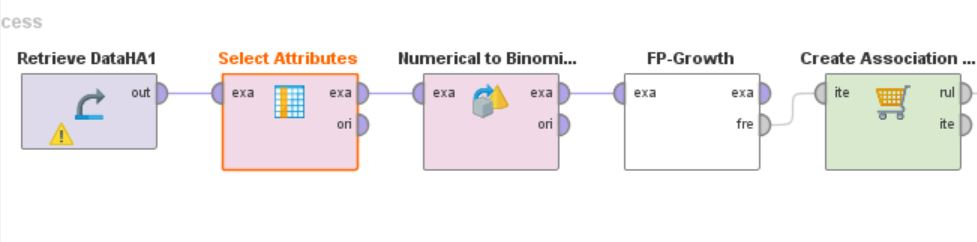
\includegraphics[width=\textwidth]{Question2Process.jpg}

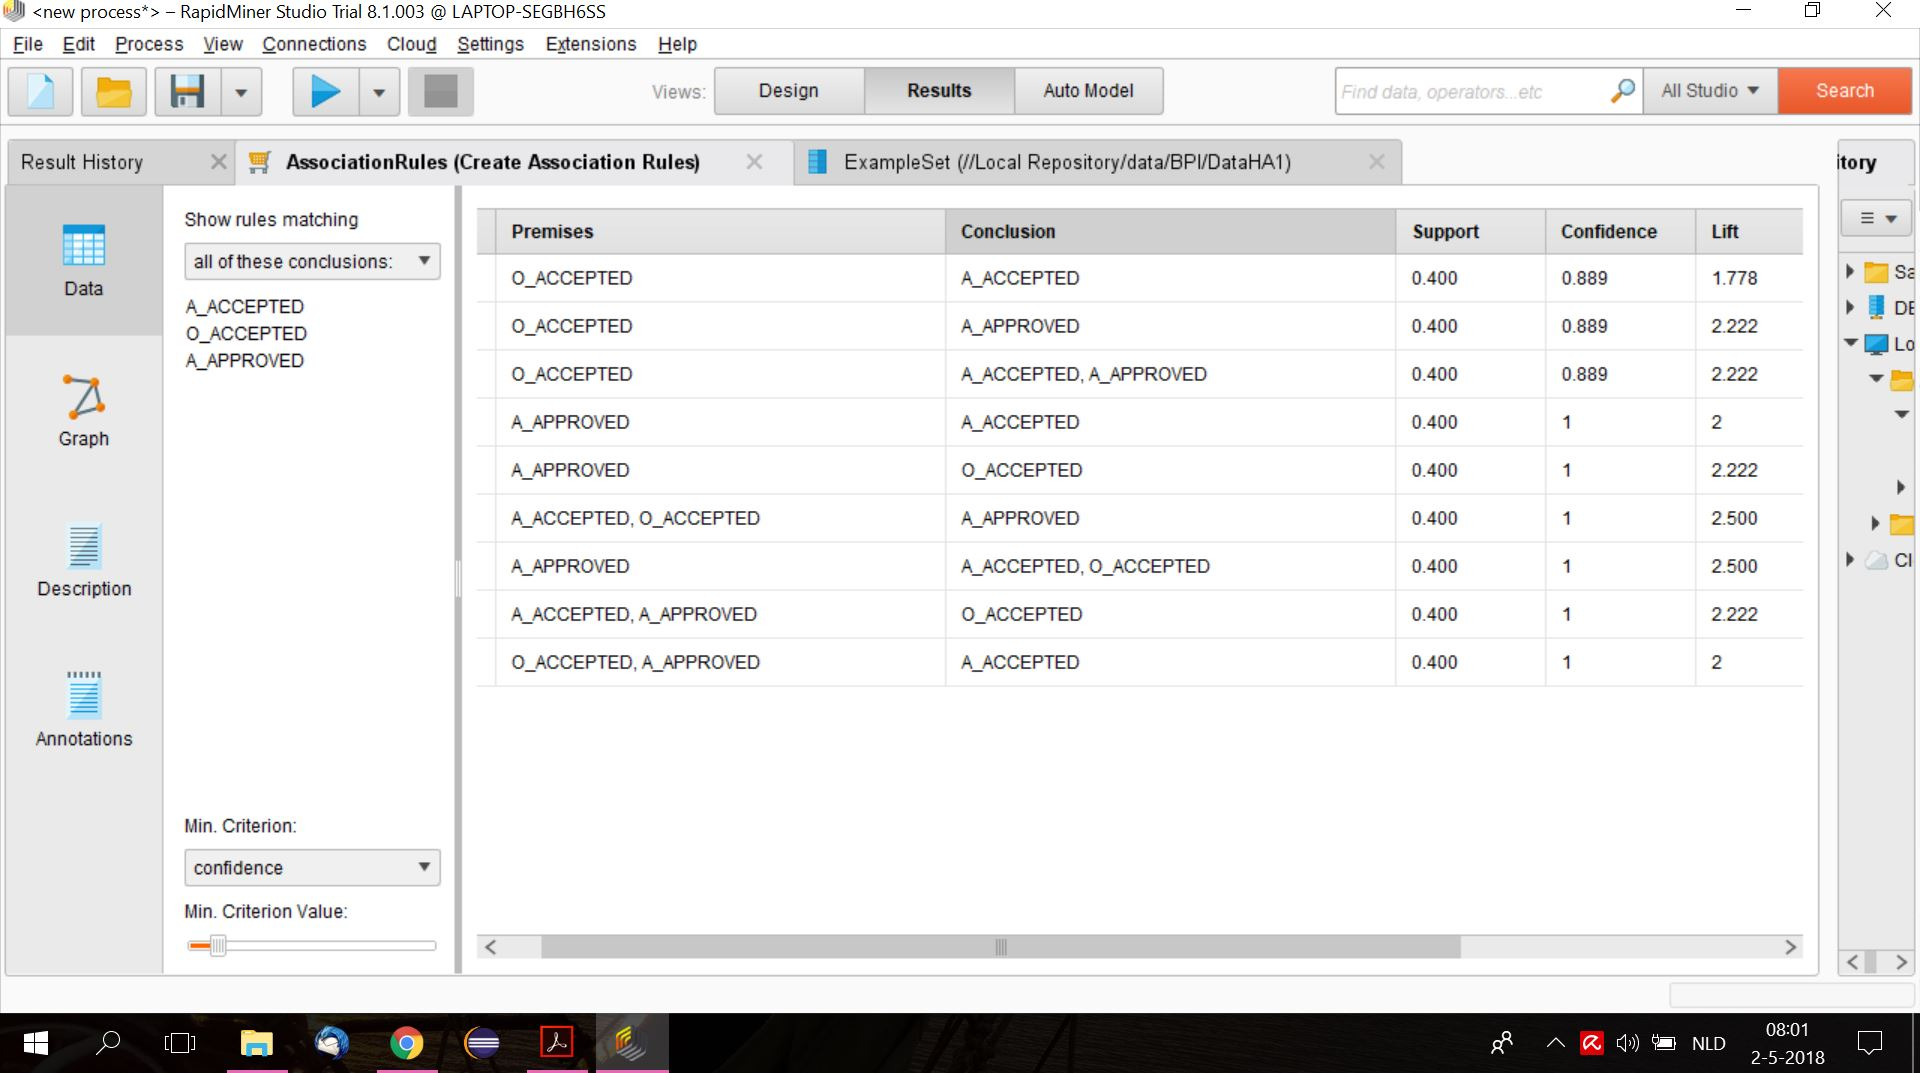
\includegraphics[width=\textwidth]{Question2Rapid.jpg}

I would pick the rule \{A\_ACCEPTED, O\_ACCEPTED\} $\Rightarrow$	\{A\_APPROVED\}
and \{A\_APPROVED\} $\Rightarrow$	\{A\_ACCEPTED, O\_ACCEPTED\}, because they
have the highest lift, confidence and support. When you have a closer look you
will see that the sets are probably of the rules have a back- and forth
relationsip. Such that you can summarize it in one rule. Then you could look for
the next best rules, where lift, support and confidence is the highest.

\section*{Question 3}
The process
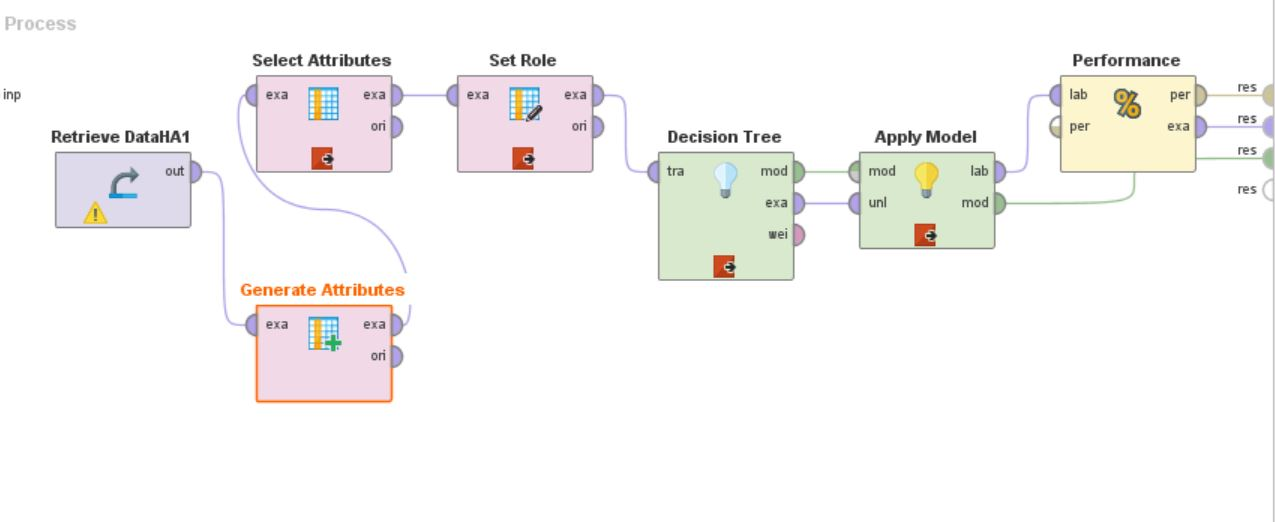
\includegraphics[width=\textwidth]{Question3Process.jpg}

first changes the numerical attribute TotalActivites to a nominal one by
\textbf{Generate Attributes} and \textbf{Select Attributes}. The generating
consideres the old TotalActivites and contains the rule that all data, where
TotalActivites is lower or the same as 40 it should be assigned to ``Low''
otherwise ``High''. The \textbf{Set Role} gives the new attribute as label, so
RapidMiner knows what should have be the outcome of the Decision Tree.
\textbf{Decision Tree} generates the decision Tree. Then \textbf{Apply Model}
for \textbf{Performance} checking. The output is then the model and the
performance of the model on the data.

The found decision tree is 

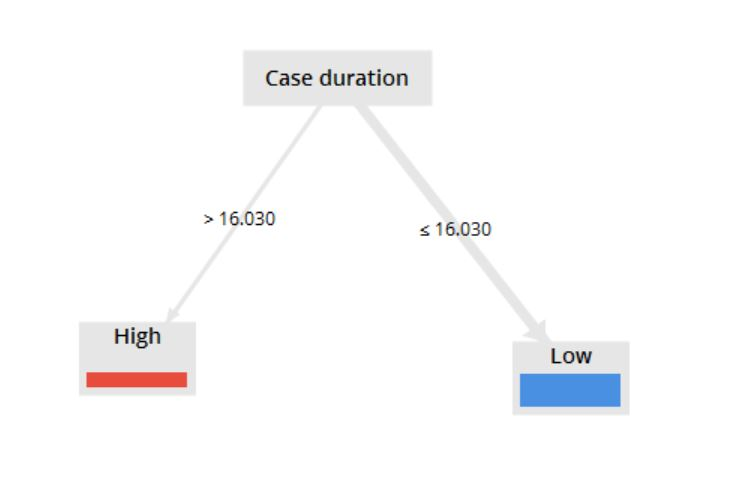
\includegraphics[width=\textwidth]{Question3Deci.jpg}

If you check the Confusionmatrix

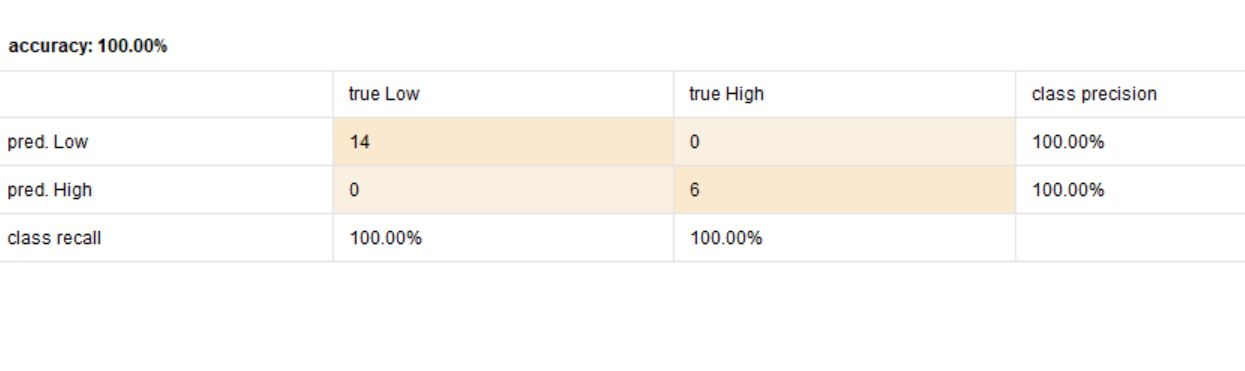
\includegraphics[width=\textwidth]{Question3Confusion.jpg}

you see, that this decision tree classifys the data perfectly. So you can
predict by just knowing the case duration the total activities. If the case
duration is higher, than also the total activities are high. This seems to be
logical, if you have to do a lot this takes most of the times longer and
otherwise around, if you do not need long you mostly did not do a lot of
different things in the time.
\section*{Question 4}
\subsection*{1.}
\begin{equation*}
L1= [\langle a,b,e,f\rangle ,\langle a,b,e,c,d,b,f\rangle ,\langle a,b,c,e,d,b
,f\rangle ,\langle a,b,c,d,e,b,f\rangle ,\langle a,e,b,c,d,b,f\rangle ]
\end{equation*}
The $\alpha-$Algorithm gives the following:

\begin{align*}
T_L &= \{ a,b,c,d,e,f\}\\
T_I &= \{a\}\\
T_O &= \{f\}
\end{align*}
\begin{tabular}{c | c c c c c c}
	&a 	  &b 			 &c 			&d 	  			&e 			   &f\\
	\hline
a	&$\#$ &$\rightarrow$ &$\#$ 			&$\#$ 			&$\rightarrow$ &$\#$\\
b	&$\leftarrow$ &$\#$			 &$\rightarrow$ &$\leftarrow$ 			&$||$ 		  
&$\rightarrow$\\
c	&$\#$ &$\leftarrow$			 &$\#$			&$\rightarrow$  &$||$ 		   &$\#$\\
d	&$\#$ &$\rightarrow$ &$\leftarrow$			&$\#$			&$||$ 		   &$\#$\\
e	&$\leftarrow$ &$||$ 		 &$||$			&$||$  			&$\#$		   &$\rightarrow$\\
f	&$\#$ &$\leftarrow$	 &$\#$			&$\#$			&$\leftarrow$		   &$\#$\\
\end{tabular}

\begin{align*}
X_L &= \{ (\{a\},\{b\}),(\{a\},\{c\})
,(\{a\},\{e\}),(\{b\},\{d\}),(\{c\},\{d\}),(\{e\},\{f\}),(\{a,e\},\{f\}),(\{f\},\{d\}),(\{a,e\},\{f,d\}),(\{a,e,f\},\{d\}),(\{e\},\{h\}),(\{e,h\},\{d\}),(\{a,e,h\},\{d\}),(\{a,e,h,f\},\{d\}),(\{e\},\{g\}),(\{g\},\{d\}),(\{e,g\},\{d\}),(\{a,e,h\},\{d\}),(\{a,e,h,g\},\{d\}),(\{a,e,h,f\},\{d\}),(\{a,e,h,f,g\},\{d\})\}\\
Y_L &=
\{(\{a\},\{b\}),(\{a\},\{c\}),(\{b\},\{d\}),(\{c\},\{d\}),(\{a,e,h,f,g\},\{f\}),(\{a,d\},\{b\})\}\\
\end{align*}

\begin{tikzpicture}[node distance=1.3cm,>=stealth',bend angle=45,auto]

  \tikzstyle{place}=[circle,thick,draw=blue!75,fill=blue!20,minimum size=6mm]
  \tikzstyle{transition}=[rectangle,thick,draw=black!75,
  			  fill=black!20,minimum size=4mm]

  \tikzstyle{every label}=[red]

  \begin{scope}
    % First net
    \node [place,tokens=1] (start)                {};
    \node [transition] (a) [right of=start]       {a}
    	edge [pre] (start);
    \node [place] (toe)  [above right of=a]	  	  {}
    	edge [pre] (a);
    \node [place] (tob) [right of=a]        {}
    	edge [pre] (a);
    \node [transition] (e) [right of=toe]         {e}
    	edge [pre] (toe);
	\node [transition] (b) [right of=tob]         {b}
		edge [pre] (tob);
    \node [place] (etof) [right of=e] {}
    	edge [pre] (e);
    \node [place] (btof) [right of=b] {}
    	edge [pre] (b);
    \node [transition] (f) [right of=etof] {f}
    	edge [pre] (btof)
    	edge [pre] (etof);
    \node [place] (end) [right of=f] {}
    	edge [pre] (f);
    \node [place] (btoc) [below right of=b] {}
    	edge [pre] (b);
    \node [transition] (c) [below right of=btoc] {c}
    	edge [pre] (btoc);
    \node [place] (ctod) [below of=b] {}
    	edge [pre] (c);
    \node [transition] (d) [below of=a] {d}
    	edge [pre] (ctod)
    	edge [post] (tob);
  \end{scope}
\end{tikzpicture}

\subsection*{2.}
\begin{equation*}
L2= [\langle a,b,c,d\rangle ,\langle a,c,b,d\rangle,\langle a,e,f,d\rangle
,\langle a,e,g,d\rangle ,\langle a,e,h,d\rangle]
\end{equation*}
The $\alpha-$Algorithm gives the following:

\begin{align*}
T_L &= \{ a,b,c,d,e,f,g,h\}\\
T_I &= \{a\}\\
T_O &= \{d\}
\end{align*}
\begin{tabular}{c | c c c c c c c c}
	&a 	  		  &b 			 &c 			&d 	  			&e 			   &f			&g			&h\\
	\hline
a	&$\#$ 		  &$\rightarrow$ &$\rightarrow$	&$\#$ 			&$\rightarrow$ &$\#$		&$\#$
   	&$\#$\\
b	&$\leftarrow$ &$\#$			 &$||$ 			&$\rightarrow$	&$\#$ 		   &$\#$		&$\#$	
	&$\#$\\
c	&$\leftarrow$ &$||$			 &$\#$			&$\rightarrow$  &$\#$ 		   &$\#$		&$\#$	
	&$\#$\\
d	&$\#$ 		  &$\leftarrow$  &$\leftarrow$	&$\#$			&$\#$ 		   &$\leftarrow$
	&$\leftarrow$ &$\leftarrow$\\
e	&$\leftarrow$ &$\#$ 		 &$\#$			&$\#$  			&$\#$		   &$\rightarrow$
	&$\rightarrow$	&$\rightarrow$\\
f	&$\#$ 		  &$\#$			 &$\#$			&$\rightarrow$	&$\leftarrow$  &$\#$		&$\#$     
&$\#$\\
g	&$\#$ 		  &$\#$			 &$\#$			&$\rightarrow$	&$\leftarrow$  &$\#$		&$\#$     
&$\#$\\
h	&$\#$ 		  &$\#$			 &$\#$			&$\rightarrow$	&$\leftarrow$  &$\#$		&$\#$     
&$\#$\\
\end{tabular}

\begin{align*}
X_L &= \{ (\{a\},\{b\}),(\{a\},\{c\})
,(\{a\},\{e\}),(\{a\},\{b,e\}),(\{a\},\{c,e\}),(\{b\},\{c\}),(\{b\},d\}),(\{c\},\{b\}),\\
&(\{c\},\{d\}),(\{e\},\{f\}),(\{e\},\{g\}),(\{e\},\{h\}),(\{g\},\{d\}),(\{h\},\{d\}),(\{f\},\{d\}),\\
&(\{g,h\},\{d\}),(\{g,f\},\{d\}),(\{h,f\},\{d\}),(\{g,f,h\},\{d\})\}\\
Y_L &= \{(\{a\},\{b,e\}),(\{a\},\{c,e\}),(\{g,f,h\},\{d\})\}\\
\end{align*}

\begin{tikzpicture}[node distance=1.3cm,>=stealth',bend angle=45,auto]

  \tikzstyle{place}=[circle,thick,draw=blue!75,fill=blue!20,minimum size=6mm]
  \tikzstyle{transition}=[rectangle,thick,draw=black!75,
  			  fill=black!20,minimum size=4mm]

  \tikzstyle{every label}=[red]

  \begin{scope}
    % First net
    \node [place,tokens=1] (start)                {};
    \node [transition] (a) [right of=start]       {a}
    	edge [pre] (start);
    \node [place] (toeb)  [above right of=a]	   {}
    	edge [pre] (a);
    \node [place] (toec) [below right of=a]        {}
    	edge [pre] (a);
    \node [transition] (e) [below right of=toeb]    {e}
    	edge [pre] (toec)
    	edge [pre] (toeb);
	\node [transition] (b) [above of=e]         {b}
		edge [pre] (toeb);
	\node [transition] (c) [above of=b]         {c}
		edge [pre] (toec);
    \node [place] (etofgh) [right of=e] {}
    	edge [pre] (e);
    \node [transition] (f) [right of=etofgh] {f}
    	edge [pre] (etofgh);
    \node [transition] (g) [below of=f] {g}
    	edge [pre] (etofgh);
    \node [transition] (h) [below of=g] {h}
    	edge [pre] (etofgh);
    \node [transition] (h) [below of=g] {h}
    	edge [pre] (etofgh);
    \node [place] (tod) [above right of=f] {}
    	edge [pre] (b)
    	edge [pre] (c)
    	edge [pre] (g)
    	edge [pre] (h)
    	edge [pre] (f);
    \node [transition] (d) [right of=tod] {d}
    	edge [pre] (tod);	
    \node [place] (end) [right of=d] {}
    	edge [pre] (d);
  \end{scope}
\end{tikzpicture}

\subsection*{r.}
\begin{equation*}
L3= [\langle d,c,b,e,f\rangle ,\langle a,e,f\rangle,\langle d,b,b,c,ef\rangle
,\langle a,b,c,d,e,f\rangle ,\langle b,d,a,c,f\rangle]
\end{equation*}
The $\alpha-$Algorithm gives the following:

\begin{align*}
T_L &= \{ a,b,c,d,e,f\}\\
T_I &= \{a,b,d\}\\
T_O &= \{f\}
\end{align*}
\begin{tabular}{c | c c c c c c c c}
	&a 	  		  &b 			 &c 			&d 	  			&e 			   &f	\\
	\hline
a	&$\#$ 		  &$\rightarrow$ &$\rightarrow$	&$\leftarrow$ 	&$\rightarrow$ &$\#$\\
b	&$\leftarrow$ &$||$			 &$||$ 			&$||$			&$\rightarrow$ &$\#$	\\
c	&$\leftarrow$ &$||$			 &$\#$			&$\||$  &$\rightarrow$ &$\rightarrow$\\
d	&$\rightarrow$&$||$  		 &$||$			&$\#$			&$\rightarrow$ &$\#$\\
e	&$\leftarrow$ &$\leftarrow$	 &$\leftarrow$	&$\leftarrow$	&$\#$
&$\rightarrow$\\
f	&$\#$ 		  &$\#$			 &$\leftarrow$			&$\#$	&$\leftarrow$  &$\#$	\\   
&$\#$\\
\end{tabular}

\begin{align*}
X_L &= \{ (\{a\},c\}),(\{a\},\{e\})
,(\{c\},\{e\}),(\{c\},\{f\}),(\{e\},\{f\}),(\{d\},\{a\}),(\{d\},\{e\})\}\\
Y_L &= X_L\\
\end{align*}

\begin{tikzpicture}[node distance=1.3cm,>=stealth',bend angle=45,auto]

  \tikzstyle{place}=[circle,thick,draw=blue!75,fill=blue!20,minimum size=6mm]
  \tikzstyle{transition}=[rectangle,thick,draw=black!75,
  			  fill=black!20,minimum size=4mm]

  \tikzstyle{every label}=[red]

  \begin{scope}
    % First net
    \node [place,tokens=1] (start)                {};
    \node [transition] (a) [below right of=start]       {a}
    	edge [pre] (start);
    \node [transition] (d) [right of=start]       {d}
    	edge [pre] (start);
    \node [transition] (b) [above right of=start]       {b}
    	edge [pre] (start);
    \node [place] (tode)  [right of=d]	   {}
    	edge [pre] (d)
    	edge [post] (a);
    \node [place] (toae) [right of=a]        {}
    	edge [pre] (a);
    \node [transition] (e) [right of=tode]    {e}
    	edge [pre] (tode)
    	edge [pre] (toae);
	\node [transition] (c) [right of=toae]        {c}
		edge [pre] (toae);
    \node [place] (etof) [right of=e] {}
    	edge [pre] (e);
    \node [transition] (f) [right of=etof] {f}
    	edge [pre] (etof);
    \node [place] (ctoe) [right of=c] {}
    	edge [pre] (c)
    	edge [post] (e);
    \node [place] (tof) [below right of=c] {}
    	edge [pre] (c)
    	edge [post] (f);
    \node [place] (end) [right of=f] {}
    	edge [pre] (f);
  \end{scope}
\end{tikzpicture}
\section*{Question 5}
\subsection*{a)}
% How many process instances and events are in this event log? What is the median
% number of events in each trace and what is the average duration of them?
The process has 150370 cases and 561470 events. Median number of events is 5.
The average duration is 48.8 weeks.

\subsection*{b)}
% What will be the Disco process model for this event log when you set Activities
% slider to 80% and Paths slider to 10%? Interpret the (self-loop) edge from
% �Payment� to itself. How many times and for how many process instances this
% behavior happens?

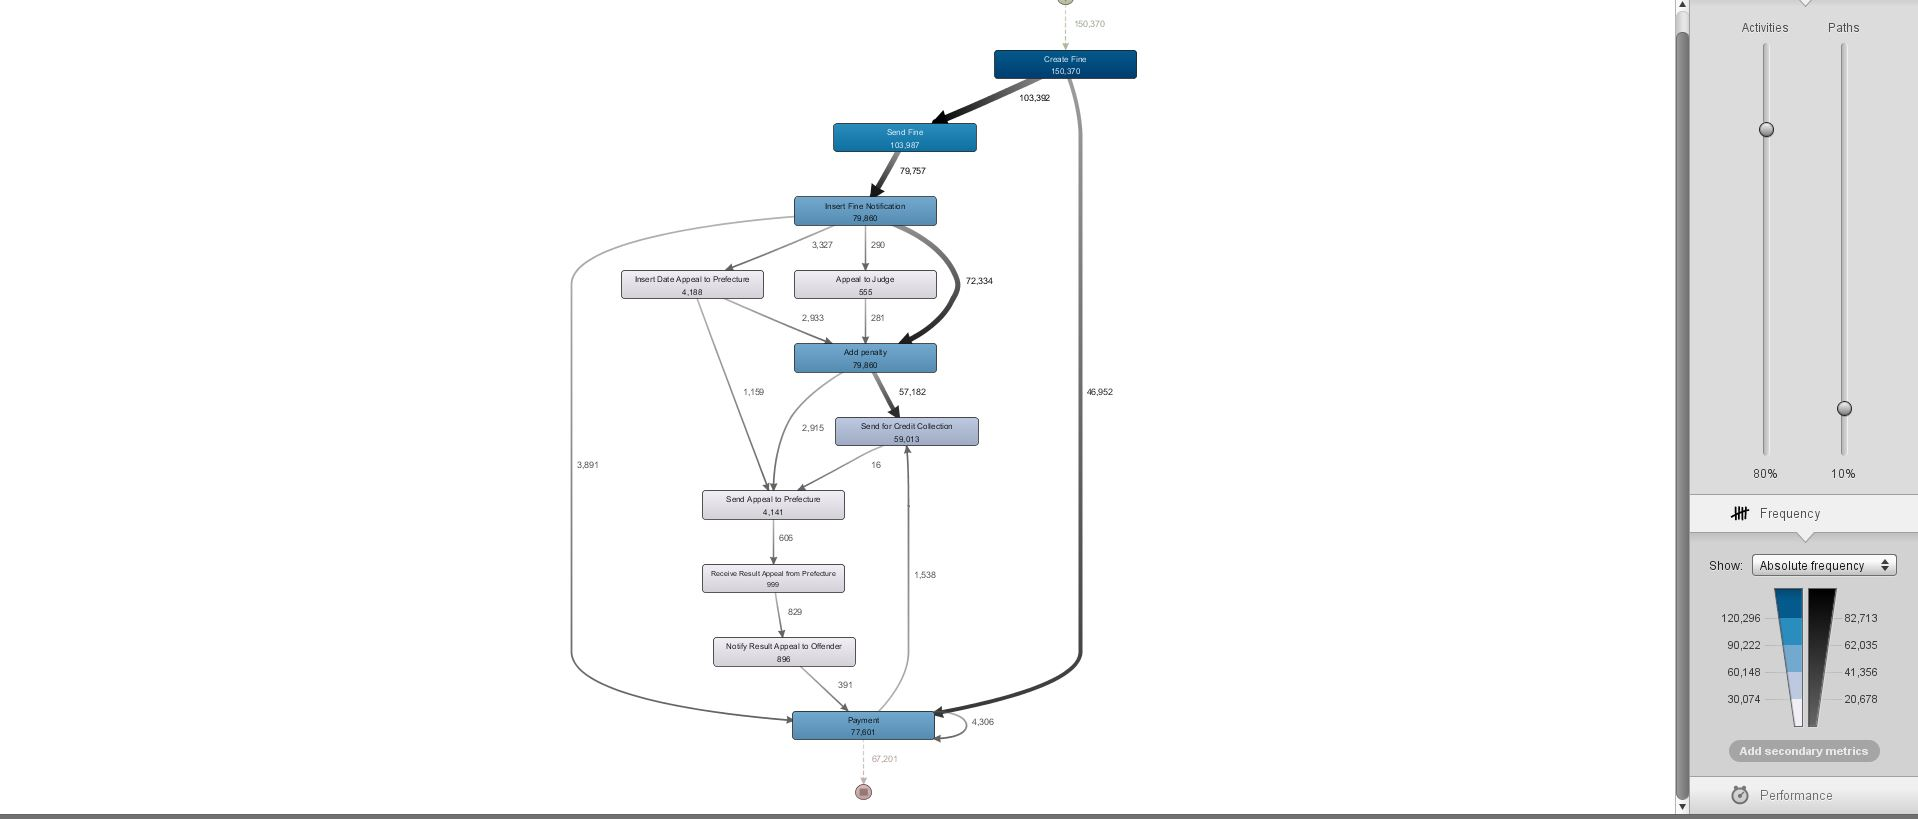
\includegraphics[width=0.8\textwidth]{Question5b.jpg}

The loop tells us, that a part of all people paid at least two times. If
you check the log data, you can see, that mostly it happens in the next 30 days.
Maybe they had a plan how to pay over weeks or had to pay penaltys.

This behavior happens 4306 and for 4014 cases. So there are cases, where it
happens more than one time. You also can see, that it happens at most 14 times.

\subsection*{c)}
%Using Disco, analyze the time distribution of events over the time covered by this
%log? What is your interpretation of the distribution of events over the time?
% Do you see any remarkable patterns in the distribution of events (drifts, repeating
%behavior, etc.)?
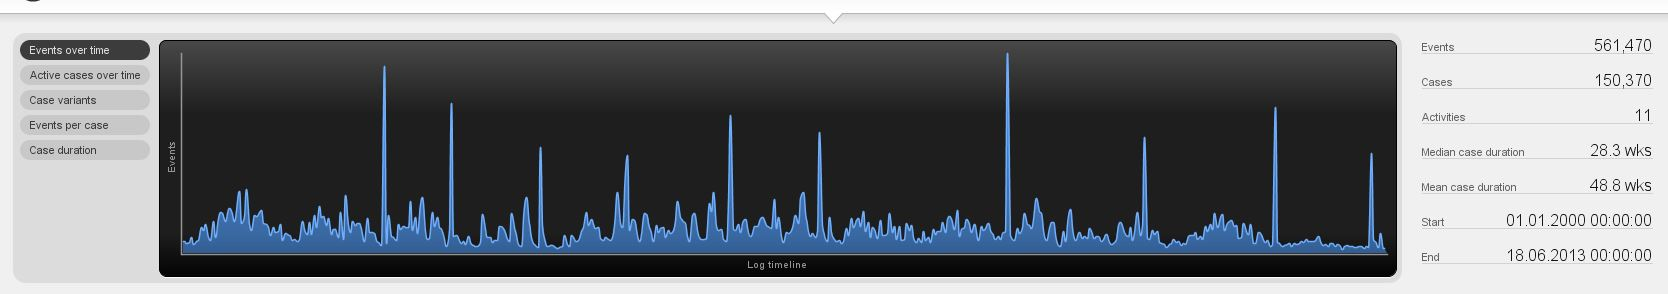
\includegraphics[width=0.8\textwidth]{Question5cDist.jpg}

You can see that the distribution is going up and down a little bit, but there
are 10 peaks to see where more happens. In the end activity gets
lower and the distance between the 6th and 7th peak is higher than between the
others.
It is always close to typical paydays, so maybe a lot of people then have
the money to pay the fine. It is also striking, that it is around the weekend.
Could be that there are more people riding too hard or just more people riding. 

The peakes are on:
06.04.2002 (Sa), 06.01.2003 (Mo), 05.01.2004 (Mo), 24.12.2004 (Fr), 20.02.2006 (Mo),
18.02.2007 (Su), 27.03.2009 (Fr), 08.10.2010 (Fr), 22.03.2012 (Thu), 19.04.2013
(Fr)

\subsection*{d)}
% How many variants are in this event log? What is the size (number of process
% instances) of the third most frequent variant? Also, explain what happens in this
% variant (report the sequence of activities).
There are 231 variants. The third most frequent variant has 20385 instances. It
just contains the behaviour \textbf{create} and \textbf{send fine}.

\subsection*{e)}
% Filter the event log using Disco while keeping 50% of the most common variants of
% process instances that finished until 01.01.2012 12: 12. What happens to the
% median and the average of case duration compared to the whole event log. Please
% also explain the difference between the median and the average (mean) of case
% duration.
It is just possible to $43\%$ or $56\%$. The average case duration shorts to
45.2 weeks from 48.8 weeks and the median to 20.9 weeks from 28.3 weeks in both
cases.
So the most common cases are in average faster finished than all cases in
average. This is like I would expect it.

The median is the instance in the middel. So if you write down all instances
sorted, it is the middel one. The average is the sum of all instances
divided by the number of instances. The average can change a lot for big or
extree small oultiers. The median shows more a real duration in the middle of
all instance durations.

\subsection*{f)}
% Discover the dotted chart view of the event log and interpret it using ProM. Adjust
% the Dotted chart settings in a way to answer question c. Are there any interesting
% (or odd) patterns in the dotted chart view that could explain the patterns found
% when answering question c?
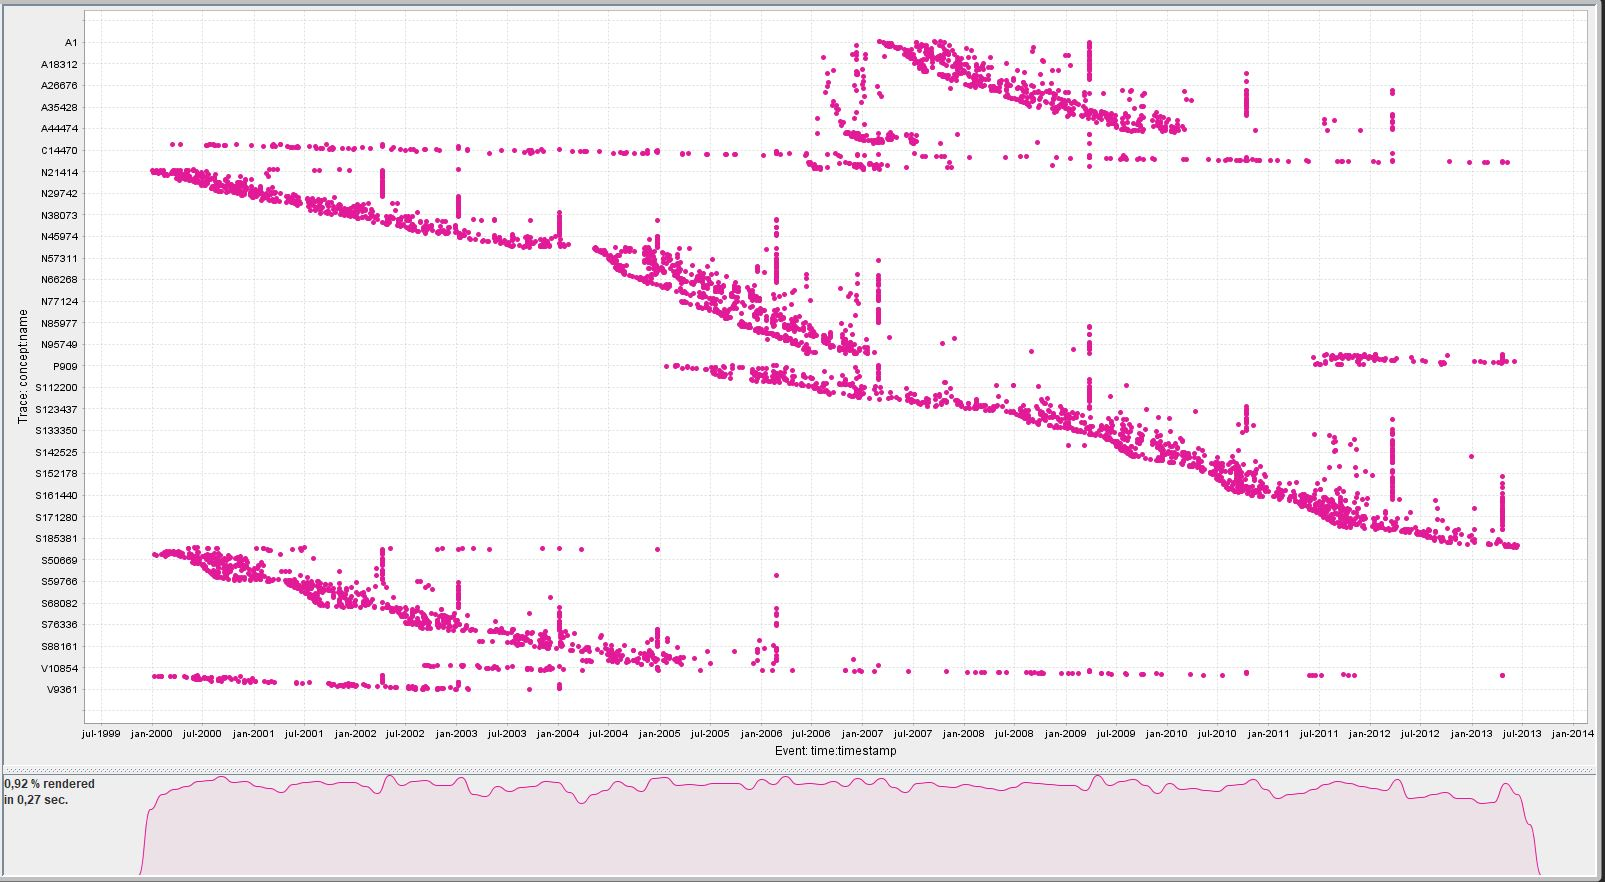
\includegraphics[width=\textwidth]{Question5f.jpg}

In the first dotted chart you see on what time which case is active.

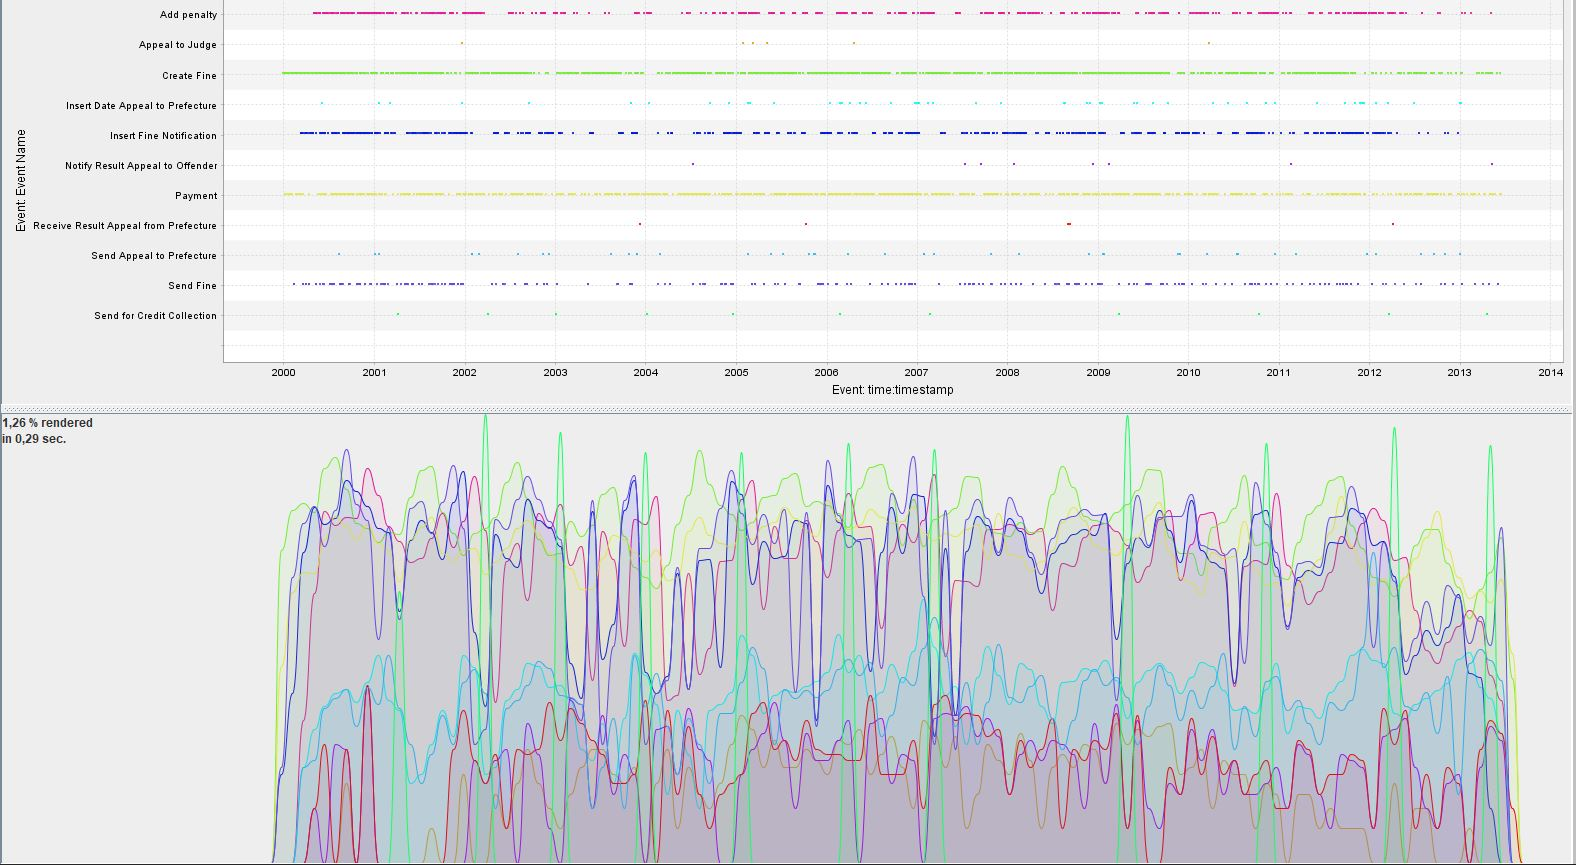
\includegraphics[width=\textwidth]{Question5fcZoomedIn.jpg}

For interpreting the dot chart for the question c) I changed the y-axis to the
event names so I can see when which events happen a lot and also coloured the
events.

For checking what exactly happens on the peaks I zoomed in (not to see in the
screenshot).

You can see that \textbf{Send for Credit Collection} is strongly connected to
the peakes to see in c). 

Payment happens close to always, but still it is a little bit bundled at the
peaks.

Furthermore I would say, that in disco it is more easy to see when peaks happen,
but in prom better to see what is happening on the peak days.

\subsection*{g)}
% Filter the event log using �filter log using simple heuristics� and then apply the
% Alpha algorithm (Alpha ++) on it. Filter the log appropriately. Show some insights
% that can only be seen after filtering.

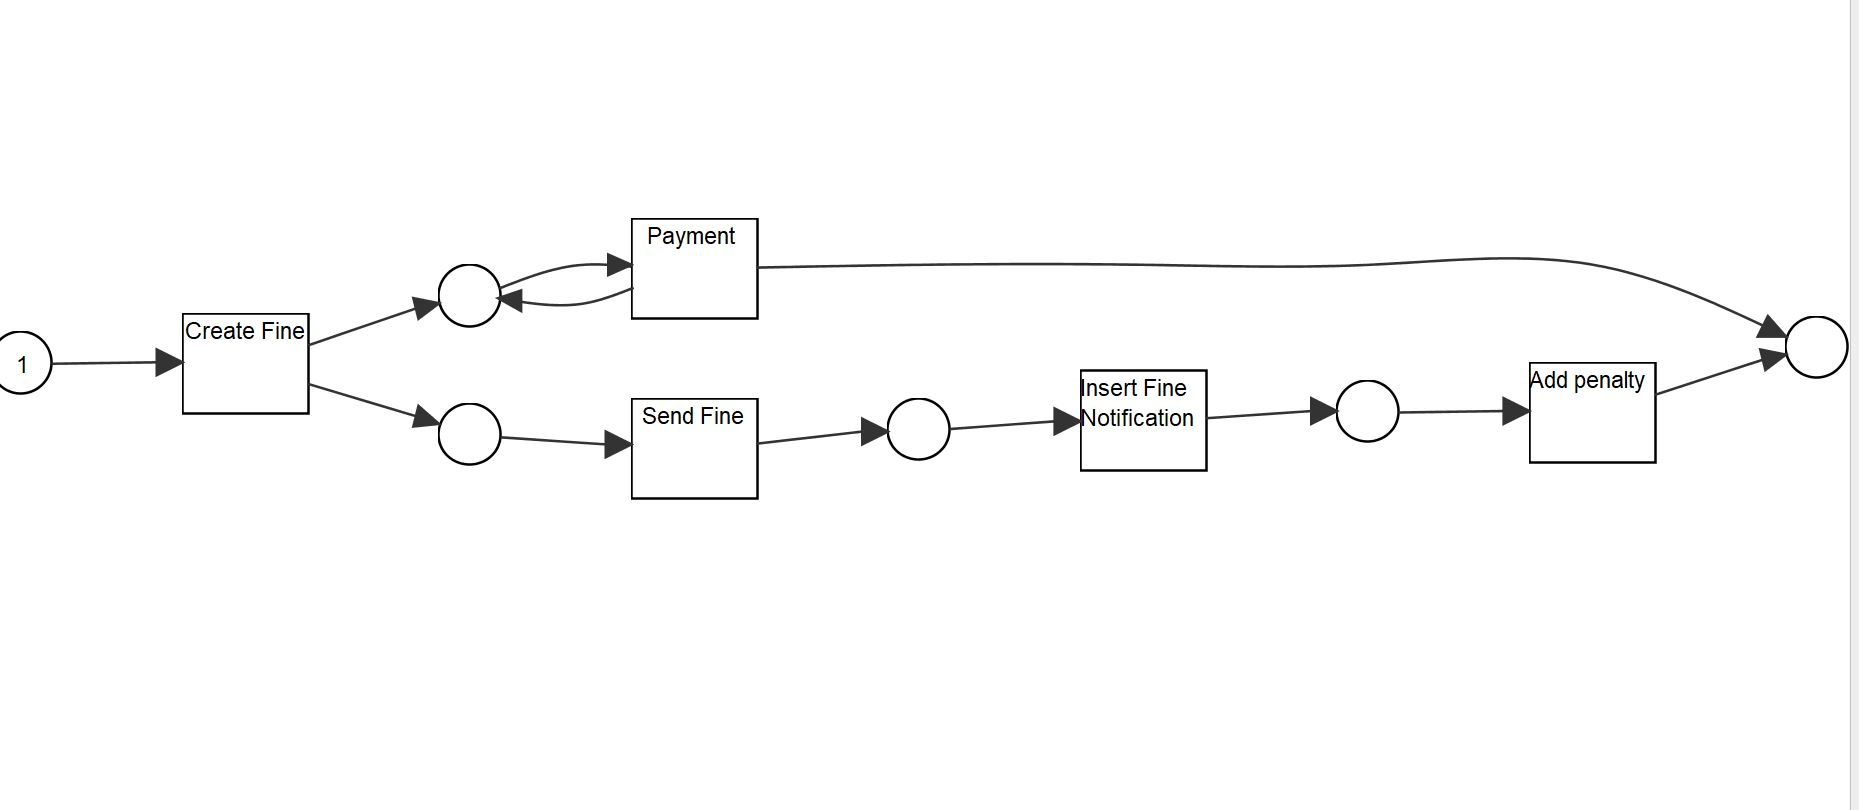
\includegraphics[width=\textwidth]{Question5g.jpg}

The filtering happened in the first case with basis settings. So 80\% of all
steps asked.
(2nd step log filter (end) just payment and send for credit, 3rd (event) add
penalty,create fine, insert fine notification, payment, send fine)

If you apply the alpha-algoirthm on the not filtered data you can not clearly
see in the resulting net, that the payment can happen always and also infinite
often. It sounds weird, because you do not expect someone paying before he gets
the fine, but looking at the data it happens.

I also filtered with different settings(, but did not have enough insights
about the data)
\begin{enumerate}
  \item 90\% for create fine and complete and choosing all end events with 80\%
  and including all events with 80\%\\
  \item 50\% for create fine+complete rest like basis\\
  \item and a few more not safed
\end{enumerate}

The alpha-algorithm used for this different setting does not give more
insights, so I does not include screenshots of it. (The data is foundable in my
filesystem)

\subsection*{h)}
% Use the filtered event log in the previous question and this time use it as input for
% Disco. Which parts of the process are time consuming for most of the process
% instances? Answer this by interpreting the Disco model.

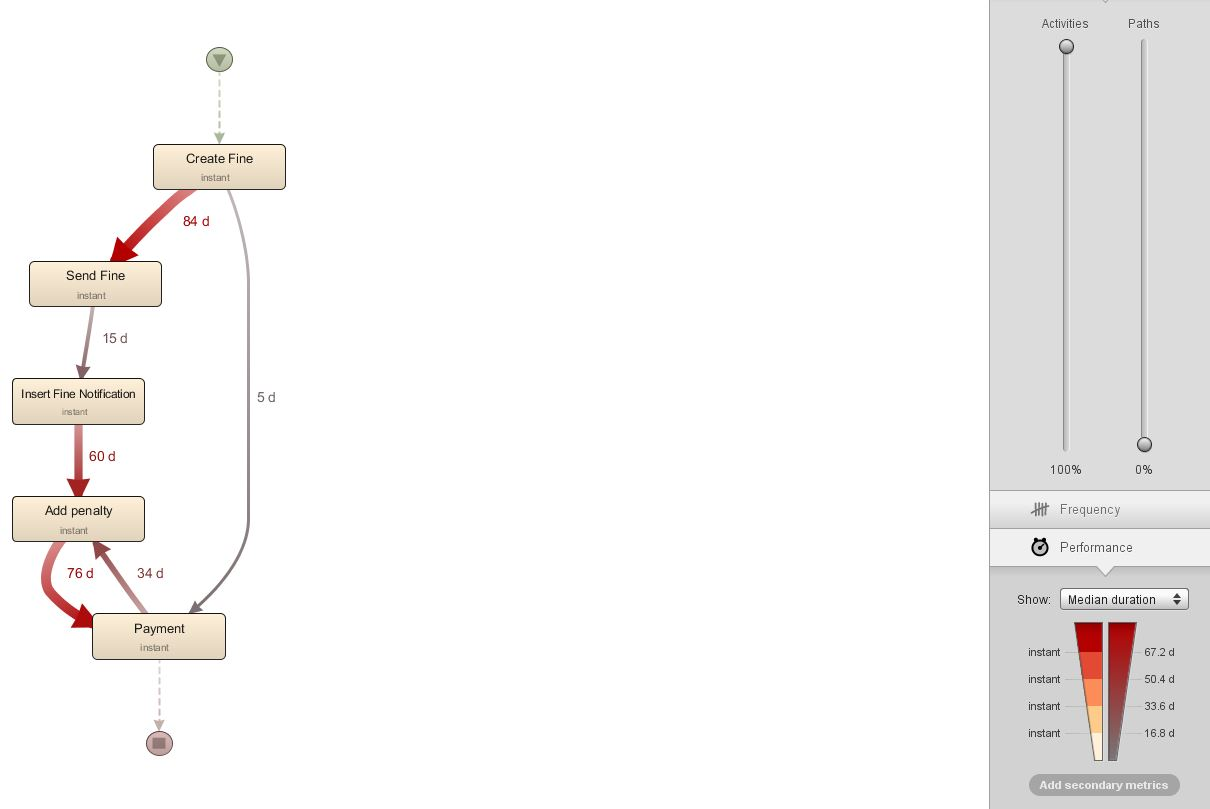
\includegraphics[width=\textwidth]{Question5h.jpg}

84days is the median for send fine. I chose the median, because then you get a
better idea what happens most of the times, because it is less exposed to
outliers.
(The biggest mean is 23.3 weeks between add penalty and payment.)

Additionaly you can see, that after exactly 60days the penalty gets
added.



\end{document}
